
\chapter{Dynamic Network Models}
% Learning and memory in the brain are implemented by complex,
% time-varying changes in neural circuitry. The computational rules
% according to which synaptic weights change over time are the subject
% of much research, and are not precisely understood. Until recently,
% limitations in experimental methods have made it challenging to test
% hypotheses about synaptic plasticity on a large scale.  However, as
% such data become available and these barriers are lifted, it becomes
% necessary to develop analysis techniques to validate plasticity
% models.  In this chapter, we present an extensible framework for modeling
% arbitrary synaptic plasticity rules on spike train data in populations
% of interconnected neurons. 

% We treat synaptic weights as a (potentially
% nonlinear) dynamical system embedded in a nonlinear autoregressive model
% of neural activity. Building on the work of preceding chapters, 
% we we show how synaptic plasticity rules can be modeled as dynamics 
% rules that govern how weights evolve in an activity-dependent manner.
% In doing so, we imbue the weights with a biophysical interpretation 
% that we explicitly avoided in previous chapters. We discuss when this
% interpretive leap is warranted. 

% To fit this model, we develop an algorithm that uses particle MCMC
% \cite{Andrieu-2010} to fit the synaptic weight trajectories alongside
% the parameters of the GLM and of the learning rules. Using this
% method, we perform model comparison of two proposed variants of the
% well-known spike-timing-dependent plasticity (STDP) rule, where
% nonlinear effects play a substantial role. On synthetic data generated
% from the biophysical simulator NEURON, we show that we can recover the
% weight trajectories, the pattern of connectivity, and the underlying
% learning rules.

%\section{Introduction}
Synaptic plasticity is believed to be the fundamental building block
of learning and memory in the brain. Its study is of crucial
importance to understanding the activity and function of neural
circuits. With innovations in neural recording technology providing
access to the simultaneous activity of increasingly large populations
of neurons, statistical models are promising tools for formulating and
testing hypotheses about the dynamics of synaptic
connectivity. Advances in optical techniques \cite{Packer-2012,
  Hochbaum-2014}, for example, have made it possible to simultaneously
record from and stimulate large populations of synaptically connected
neurons. Armed with statistical tools capable of inferring
time-varying synaptic connectivity, neuroscientists could test
competing models of synaptic plasticity, discover new learning rules
at the monosynaptic and network level, investigate the effects of
disease on synaptic plasticity, and potentially design stimuli to
modify neural networks.

Despite the popularity of autoregressive models for spike data, like 
the GLM~\cite{Paninski-2004, Truccolo-2005, Pillow-2008},
relatively little work has attempted to model the time-varying nature
of neural interactions.  Here we model interaction weights as a
dynamical system governed by parametric synaptic plasticity rules. 
% We treat synaptic weights as a (potentially
% nonlinear) dynamical system embedded in a nonlinear autoregressive model
% of neural activity. 
Building on the work of preceding chapters, 
we we show how synaptic plasticity rules can be modeled as dynamics 
rules that govern how weights evolve in an activity-dependent manner.
In doing so, we imbue the weights with a biophysical interpretation 
that we explicitly avoided in previous chapters. We discuss when this
interpretive leap is warranted. 

To perform inference in this model, we use particle Markov Chain Monte
Carlo (pMCMC) \cite{Andrieu-2010}, a recently developed inference
technique for complex time series.  We use this new modeling framework
to examine the problem of using recorded data to distinguish between
proposed variants of spike-timing-dependent plasticity (STDP) learning
rules. On synthetic data generated from the biophy sical simulator
NEURON, we show that we can recover the weight trajectories, the
pattern of connectivity, and the underlying learning rules.

\section{A Biophysical Interpretation of the GLM}
The nonlinear autoregressive models of the previous chapter 
treat the spike count,~$s_{t,n}$, as a random variable whose 
distribution depends on a non-negative firing rate,~$\lambda_{t,n}$.
The firing rate is modeled as a nonlinear function of an activation,~$\psi_{t,n}$,
which is taken to be a linear function of the spike history.
This linear-nonlinear cascade is often called a generalized linear model 
\cite{Paninski-2004, Truccolo-2005}.

From a biophysical perspective, the activation can be thought of as 
analogous to the cell's membrane potential. The nonlinearity that 
links the activation to the firing rate approximates the spiking 
threshold of the neuron.
 When the membrane potential exceeds the spiking threshold
potential of the cell,~$\lambda_{t,n}$ rises to reflect the rate of the
cell's spiking, and when the membrane potential decreases below the
spiking threshold,~$\lambda(t)$ decays to zero. 

As before, we model the activation, or membrane potential,
 as a linear function of the spike history,
\begin{align}
  \label{eqn:glm_rate}
  \psi_{t,n} &= \psi_n^{(0)} + \sum_{n=1}^N \sum_{d=1}^D h_{n' \to n}[d] \cdot s_{t-d, n'}.
\end{align}
where~$\psi_n^{(0)}$ is the baseline activation,  and~$h_{n'\to n}[d]$
is an impulse response that preceding spikes on
neuron~$n'$ induce on the membrane potential of neuron~$n$ at lag~$d$. 

\begin{figure}[t!]
  \centering
  \begin{subfigure}[T]{5.25in}
    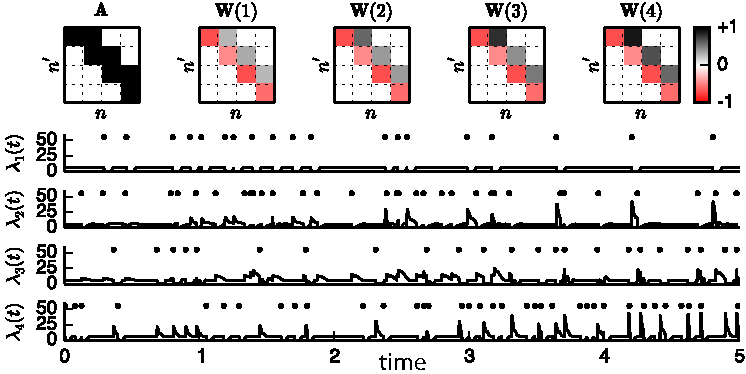
\includegraphics[width=\textwidth]{figures/ch4/figure1}    
  \end{subfigure}
  \caption[A simple example of a GLM with time-varying synaptic weights]{
    A simple network of four sparsely connected neurons whose
    synaptic weights are changing over time. Here, the neurons have
    inhibitory self connections to mimic refractory effects, and are
    connected via a chain of excitatory synapses, as indicated by the
    nonzero entries~$A_{1\to 2}$,~$A_{2 \to 3}$, and~$A_{3\to 4}$. The
    corresponding weights of these synapses are strengthening over time
    (darker entries in~$\bW$), leading to larger impulse responses in
    the firing rates and a greater number of induced post-synaptic
    spikes (black dots), as shown below.}
  \label{fig:model_illustration}
\end{figure}

From this semi-biophysical perspective it is clear that one
shortcoming of the standard GLM is that it does not account for
time-varying connectivity, despite decades of research showing that
changes in synaptic weight occur over a variety of time scales and are
the basis of many fundamental cognitive processes. This absence is
due, in part, to the fact that this direct biophysical interpretation
is not warranted in most traditional experimental regimes, e.g., in
multi-electrode array (MEA) recordings where electrodes are relatively
far apart.  However, as high resolution optical recordings grow in
popularity, this assumption must be revisited; this is a central
motivation for the present model.

There have been a few efforts to incorporate dynamics into the
GLM. \citet{Stevenson-2011} extended the GLM to take inter-spike
intervals as a covariates and formulated a generalized bilinear model
for weights. \citet{Eldawlatly-2010} modeled the time-varying
parameters of a GLM using a dynamic Bayesian network (DBN). However,
neither of these approaches accommodate the breadth of synaptic
plasticity rules present in the literature. For example, parametric
STDP models with hard bounds on the synaptic weight are not congruent
with the convex optimization techniques used by \cite{Stevenson-2011},
nor are they naturally expressed in a DBN. Here we model time-varying
synaptic weights as a potentially nonlinear dynamical system and
perform inference using particle MCMC.

Nonstationary, or time-varying, models of synaptic weights have also
been studied outside the context of GLMs. For example,
\citet{Petreska-2011} applied hidden switching linear dynamical
systems models to neural recordings. This approach has many merits,
especially in traditional MEA recordings where synaptic connections
are less likely and nonlinear dynamics are not necessarily
warranted. Outside the realm of computational neuroscience and spike
train analysis, there exist a number of dynamic statistical models,
such as \citet{West-1985}, which explored dynamic generalized linear
models. However, the types of models we are interested in for studying
synaptic plasticity are characterized by domain-specific transition
models and sparsity structure, and until recently, the tools for
effectively performing inference in these models have been limited.


\section{A Sparse Time-Varying Generalized Linear Model}
In order to capture the time-varying nature of synaptic weights, we
extend the standard GLM by first factoring the impulse responses in
the firing rate of Eq.~\ref{eqn:glm_rate} into a product of three
terms:
\begin{align}
\label{eqn:tvwglm_ir}
h_{n' \to n}[d, t] \triangleq a_{n'\to n} \cdot w_{n' \to n}[t] \cdot \hbar_{n' \to n}[d].
\end{align}
Here,~${a_{n'\to n}\in\{0,1\}}$ is a binary random variable indicating
the presence of a direct synapse from neuron~$n'$ to
neuron~$n$,~~${w_{n'\to n}[t] \in \reals}$ is a non stationary
synaptic ``weight'' trajectory associated with the synapse, and~$\hbar_{n'
  \to n}[d]$ is a nonnegative, normalized impulse response,
i.e. ~${\sum_{d=1}^D \hbar_{n' \to n}[d] \cdot \Delta t =
  1}$. Requiring~${\hbar_{n' \to n}[d]}$ to be normalized gives
meaning to the synaptic weights: otherwise~$w$ would only be defined
up to a scaling factor. For simplicity, we assume~$\hbar[d]$ does
not change over time, that is, only the amplitude and not the duration
of the PSPs are time-varying. This restriction could be adapted in
future work.

As is often done in GLMs, we model the normalized impulse responses as
a linear combination of basis functions. In order to enforce the
normalization of~$\hbar[d]$, however, we use a \emph{convex}
combination of normalized, nonnegative basis functions. That is,
\begin{align*}
\hbar_{n' \to n}[d] \equiv \sum_{b=1}^B \theta_{n' \to n}^{(b)}\, \phi_b[d],
\end{align*}
where~${\sum_{d=1}^D \phi_b[d] \cdot \Delta t = 1}$ and
${\sum_{b=1}^B \theta_{n' \to n}^{(b)} = 1}$. 

The binary random variables~$a_{n' \to n}$, which can be collected
into an~${N\times N}$ binary matrix~$\bA$, model the connectivity of
the synaptic network. Similarly, the collection of weight
trajectories~${\{\{w_{n' \to n}[t]\}\}_{n',n}}$, which we will
collectively refer to as~$\bW[t]$, model the time-varying synaptic
weights. This factorization is often called a \emph{spike-and-slab}
prior \cite{Mitchell1988}, and it allows us to separate our prior
beliefs about the structure of the synaptic network from those about
the evolution of synaptic weights. For example, in the most general
case we might incorporate the probabilistic network models of previous chapters
 as prior distributions for~$\bA$, but here we limit
ourselves to the simplest network model, the Erd\H{o}s-Renyi
model. Under this model, each~$a_{n' \to n}$ is an independent
identically distributed Bernoulli random variable with sparsity
parameter~$\rho$.

Figure~\ref{fig:model_illustration} illustrates how the adjacency
matrix and the time-varying weights are integrated into the GLM. Here,
a four-neuron network is connected via a chain of excitatory synapses,
and the synapses strengthen over time due to an STDP rule. This is
evidenced by the increasing amplitude of the impulse responses in the
firing rates.  With larger synaptic weights comes an increased
probability of postsynaptic spikes, shown as black dots in the
figure. In order to model the dynamics of the time-varying synaptic
weights, we turn to a rich literature on synaptic plasticity and
learning rules.

\subsection{Learning Rules for Time-Varying Synaptic Weights}
Decades of research on synapses and learning rules have yielded a
plethora of models for the evolution of synaptic weights
\cite{Caporale-2008}. In most cases, this evolution can be written as
a dynamical system,
\begin{align*} 
\bW[t] &= \bW[t-1] + \ell\left(\bW[t-1], \, \mcH_t, \bvartheta \right) + \epsilon(\bW[t], \bvartheta)
\end{align*}
where~$\ell$ is a potentially nonlinear \emph{learning rule} that
determines how synaptic weights change as a function of previous
spiking. This framework encompasses rate-based rules such as the Oja
rule \cite{Oja-1982} and timing-based rules such as STDP and its
variants. The additive noise,~${\epsilon(\bW(t), \bvartheta)}$, need not be
Gaussian, and many models require truncated noise distributions.

Following biological intuition, many common learning rules factor into
a product of simpler functions. For example, STDP (defined below)
updates each synapse independently such that the learning rule for 
~$w_{n' \to n}$ only
depends on~${w_{n'\to n}[t-1]}$ and the presynaptic spike
history~${\bs_{1:t-1,n}}$. Biologically speaking, this means that
plasticity is local to the synapse. More sophisticated rules allow
dependencies among the columns of~$\bW$. For example, the incoming
weights to neuron~$n$ may depend upon one another through
normalization, as in the Oja rule \cite{Oja-1982}, which scales
synapse strength according to the total strength of incoming synapses.

\sloppy 
Extensive research in the last fifteen years has identified the
relative spike timing between the pre- and postsynaptic neurons as a
key component of synaptic plasticity, among other factors such as mean
firing rate and dendritic depolarization \cite{Feldman-2012}. STDP is
therefore one of the most prominent learning rules in the literature
today, with a number of proposed variants based on cell type and
biological plausibility. In the experiments to follow, we will make
use of two of these proposed variants. First, consider the canonical
STDP rule with a ``double-exponential" function parameterized by
${\bvartheta = \{\tau_-, \tau_+, A_-, A_+\}}$ \cite{Song-2000}, in which the
effect of a given pair of pre-synaptic and post-synaptic spikes on a
weight may be written:
\begin{align}
\label{eqn:AddSTDP}
 \ell\left(w_{n' \to n}[t], \mcH_t, \bvartheta \right) &= 
 \;s_{t,n} \, \ell_+(\mcH_t, A_+, \tau_+) 
 \;-\;s_{t,n'} \, \ell_-(\mcH_t, A_-, \tau_-),
\end{align}
where,
\begin{align*}
\ell_+(\mcH_t; A_+, \tau_+) &= \sum_{t'=1}^{t-1} s_{t', n'} \cdot  A_+ \cdot e^{(t-t')/\tau_+}, \\
\ell_-(\mcH_t; A_-, \tau_-) &= \sum_{t'=1}^{t-1} s_{t', n} \cdot  A_- \cdot e^{(t-t')/\tau_-}.
\end{align*}
This rule states that weight changes only occur at the time of pre- or
post-synaptic spikes, and that the magnitude of the change is a
nonlinear function of interspike intervals.
%However, this model assumes that synaptic weights are unbounded from
%above and may change sign, both of which are implausible assumptions
%for a fixed excitatory or inhibitory neuron with saturating synaptic
%weight.  This type of model may be captured with the generalized
%bilinear model of \citet{Stevenson-2011} by treating the interspike
%intervals as covariates.

A slightly more complicated model known as the multiplicative STDP
rule extends this by bounding the weights above and below
by~$W_{\mathsf{max}}$ and~$W_{\mathsf{min}}$, respectively
\cite{Morrison-2008}. Then, the magnitude of the weight update is
scaled by the distance from the threshold:
\begin{align}
 \label{eqn:MultSTDP}
 \ell\left(w_{n' \to n}[t], \mcH_t, \bvartheta \right) = 
 \;& s_{t,n} \;  \tilde\ell_+(\mcH_t; A_+, \tau_+) \; (W_{\mathsf{max}}-w_{n'\to n}[t]), \nonumber \\
  \;-\; &s_{t,n'}\;  \tilde\ell_-(\mcH_t; A_-, \tau_-) \; (w_{n'\to n}[t]-W_{\mathsf{min}}).
\end{align}
Here, by setting ${\tilde\ell_\pm = \min(\ell_\pm,1)}$, we enforce
that the synaptic weights always fall
within~${[W_{\mathsf{min}}, W_{\mathsf{max}}]}$. With this rule, it
often makes sense to set $W_{\mathsf{min}}$ to zero.

Similarly, we can construct an additive, bounded model which is
identical to the standard additive STDP model except that weights are
thresholded at a minimum and maximum value. In this model, the weight
never exceeds its set lower and upper bounds, but unlike the
multiplicative STDP rule, the proposed weight update is independent of
the current weight except at the boundaries. Likewise, whereas with
the canonical STDP model it is sensible to use Gaussian noise
for~$\epsilon(t)$ in the bounded multiplicative model we use truncated
Gaussian noise to respect the hard upper and lower bounds on the
weights.  Note that this noise is dependent upon the current
weight,~$w_{n'\to n}[t]$.

The nonlinear nature of this rule, which arises from the
multiplicative interactions among the parameters,~${\bvartheta =
  \{A_+,\tau_+,A_-,\tau_-,W_{\mathsf{max}}, W_{\mathsf{max}}\}}$,
combined with the potentially non-Gaussian noise models, pose
substantial challenges for inference. However, the computational cost
of these detailed models is counterbalanced by dramatic expansions in
the flexibility of the model and the incorporation of \emph{a priori}
knowledge of synaptic plasticity. These learning models can be
interpreted as strong regularizers of models that would otherwise be
highly underdetermined, as there are~$N^2$ weight trajectories and
only~$N$ spike trains. In the next section we will leverage powerful
new techniques for Bayesian inference in order to capitalize on these
expressive models of synaptic plasticity.

\section{Inference via particle MCMC}
The traditional approach to inference in the standard GLM is penalized
maximum likelihood estimation. For a typical model with Poisson observations 
and an link function,~${g: \reals \to \reals_+}$, the 
log likelihood is,
\begin{align}
\label{eqn:glm_lkhd}
\log p(\bS \given \bLambda) 
  &= 
    \sum_{n=1}^N \sum_{t=1}^T  -\lambda_{t,n} \, \Delta t
    + s_{t,n} \, \log \lambda_{t,n}  \\
  &= \sum_{n=1}^N \sum_{t=1}^T  -g(\psi_{t,n}) \, \Delta t
    + s_{t,n} \, \log g(\psi_{t,n}) 
\end{align}
and the log likelihood of a population of non-interacting spike trains
is simply the sum of each of the log likelihoods for each neuron. The
likelihood depends upon the network 
through the definition of the activation given
in Eq.~\ref{eqn:glm_rate} and Eq.~\ref{eqn:tvwglm_ir}. 
% For some link functions~$g$, the log
% likelihood is a concave function of , and the
% MLE can be found using efficient optimization techniques. Certain
% dynamical models, namely linear Gaussian latent state space models,
% also support efficient inference via point process filtering
% techniques \cite{Smith-2003}.

Due to the potentially nonlinear and non-Gaussian nature of STDP,
these existing techniques are not applicable here. Instead we use
particle MCMC~\cite{Andrieu-2010}, a powerful technique for inference
in time series. Particle MCMC samples the posterior distribution over
weight trajectories,~$\bW[t]$, the adjacency matrix~$\bA$, and the
model parameters~$\btheta^{(n \to n')}$ and~$\bvartheta$, given the
observed spike trains, by combining particle filtering with MCMC.  We
represent the conditional distribution over weight trajectories with a
set of discrete particles,~${\{\bW^{(p)}\}_{p=1}^P}$. Each particle
represents a sequence of weight
matrices,~$\bW^{(p)} \in \reals^{N \times N \times T}$, and has an
associated nonnegative \emph{particle weight}~$v^{(p)}$. Note that the particle
weights are \emph{not} the same as the synaptic weights. Together,
these define an atomic distribution over weight trajectories,
\begin{align}
p(\bW) &\approx \frac{\sum_{p=1}^P v_p \, \delta_{\bW^{(p)}} (\bW)}
         {\sum_{p=1}^P v_p},
\end{align}
where~$\delta_{w*}(w)$ is the Dirac delta function located at~$w^*$.

\subsection{Particle Filtering}
Particle filtering \cite{andrieu2003introduction} or \emph{sequential
  Monte Carlo} is a method of inferring a distribution over weight
trajectories by iteratively propagating forward in time and
reweighting according to how well the new samples explain the data.
We build up the collection of weight trajectories iteratively, one
time bin at a time. We start by sampling the initial synaptic weights
from the prior distribution,
\begin{align*}
  \bW^{(p)}[1] &\sim p(\bW \given \bvartheta),
\end{align*}
and initializing the particle weights to~${v_1^{(p)} = \frac{1}{P}}$.
Then, we iteratively proceed, updating the synaptic weights according to the 
learning rule and updating the particle weights according to the likelihood 
of the spikes. That is, for~${t=2, \ldots, T}$, we perform the following steps:
\begin{enumerate}
\item Sample the next synaptic weight given the weight in the
  preceding time bin, the learning rule, the spike history, and the
  global parameters,
  \begin{align*}
    \bW^{(p)}[t] &\sim p(\bW[t] \given \bW^{(p)}[t-1], \mcH_t, \bvartheta).
  \end{align*}

\item Compute the likelhood of the current spikes,
  \begin{align*}
    \alpha_t^{(p)} &= p(\bs_t \given \bA, \bW^{(p)}[t], \{\btheta_{n \to n'}\}, \{\psi_n^{(0)}\}, \mcH_t )
  \end{align*}
\item Update the particle weight according to the likelhood of the current spikes,
  \begin{align*}
    v_t^{(p)} &\from v_{t-1}^{(p)} \cdot \alpha_t^{(p)}.
  \end{align*}
\end{enumerate}
This is, in fact, a special case of \emph{sequential importance sampling} where
our synaptic weights are sampled from the model's learning rule.

The problem with this simple algorithm is that the weights will rapidly 
decay to zero as particles drift from the regions of high likelihood. 
To counteract this effect, we often introduce a third step in which we 
\emph{resample} the particles with replacement according to their weights. 
\begin{enumerate}
\item[4.] Sample new particle indices with replacement according to the current weights, 
  \begin{align*}
    p' &\sim \distCategorical \left(
         \left[ \frac{v^{(1)}}{\sum_{p} v^{(p)}}, \ldots,
         \frac{v^{(P)}}{\sum_{p} v^{(p)}} \right] \right),
  \end{align*}
  and then replace the weights with the particle indices,
  \begin{align*}
    \bW^{(p)}[1,\ldots,t] &\from \bW^{(p')}[1,\ldots,t].
  \end{align*}

\item[5.]   Once we have resampled the particle indices, we can reset the weights.
  \begin{align*}
    v_t^{(p)} &\from \frac{1}{P}.
  \end{align*}
\end{enumerate}
This is called \emph{sequential importance resampling}. At the end of~$T$
time steps we are left with a weighted set of synaptic weight trajectories
that approximates the conditional distribution over synaptic weights 
for given global model parameters.

\subsection{Collapsed Gibbs Sampling of $\bA$ and $\bW[t]$}
The particle weights also provide an unbiased estimate of the marginal
likelihood of entries in the adjacency matrix,~$\bA$, integrating out
the corresponding weight trajectory. We have,
\begin{align*}
p(\bA \given & \bS, \{\btheta_{n \to n'}\}, \{\psi_n^{(0)}\}) \\
&\propto  \sum_{t=1}^{T} \int  p( \bA, \bW[t] \given \bS, \{\btheta_{n \to n'}\}, \{\psi_n^{(0)}\}) \, \mathrm{d}\bW[t] \\
&\approx \left[\prod_{t=1}^T \sum_{p=1}^P v_t^{(p)} \alpha_t^{(p)} \right] p(\bA \given \{\bz_n\}, \bvartheta).
\end{align*}
We can leverage this estimator in a particle marginal Metropolis-Hastings
\cite{Andrieu-2010} update. First, we propose an update to~$\bA$, then
we run a particle filter to estimate the marginal likelihood of~$\bA$, 
and accept or reject the proposal accordingly.
By marginalizing out the weight trajectory, we
are able to explore the space of adjacency matrices more efficiently.

\paragraph{Factored Learning Rules}
If the learning rule factors into
independent updates for each~$W_{n' \to n}[t]$, we can update
each synapse's weight trajectory separately and reduce the particles
to one-dimensional trajectories. The STDP learning rules considered 
in this chapter all factor in this way. 


\subsection{Particle MCMC}
Particle filtering only yields a distribution over weight
trajectories, and implicitly assumes that the other parameters have
been specified. Particle MCMC provides a broader inference algorithm
for both weights and static parameters. The idea is to interleave
\emph{conditional} particle filtering steps that sample the weight
trajectory given the current model parameters and the previously
sampled weights, with traditional Gibbs updates to sample the model
parameters given the current weight trajectory. This combination
leaves the stationary distribution of the Markov chain invariant and
allows joint inference over weights and parameters.  

In our implementation, we also make use of
a pMCMC variant with ancestor sampling~\cite{Lindsten-2012} that
significantly improves convergence. Any distribution may be used to
propagate the particles forward; using the learning rule is simply the
easiest to implement and understand.  We have omitted a number of
details in this description; for a thorough overview of particle MCMC,
the reader should consult \cite{Andrieu-2010, Lindsten-2012}.



\section{Evaluation}

\begin{figure}[t!]
  \centering
  \vspace{-0.5em}
  \begin{subfigure}[T]{2.4in}
    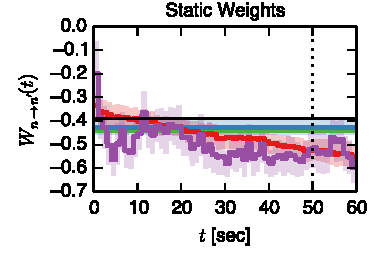
\includegraphics[width=\textwidth]{figures/ch4/fig3_static_trajectory}    
    \label{fig:fig3_static_trajectory}
  \end{subfigure}
  \begin{subfigure}[T]{1.45in}
    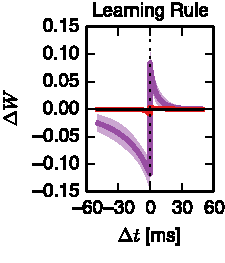
\includegraphics[width=\textwidth]{figures/ch4/fig3_static_stdp_rule}    
    \label{fig:fig3_static_stdp_rule}
  \end{subfigure}
  \begin{subfigure}[T]{1.45in}
    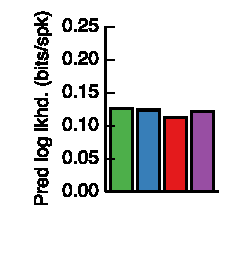
\includegraphics[width=\textwidth]{figures/ch4/fig3_static_pred_ll}    
    \label{fig:fig3_static_pred_ll}
  \end{subfigure} \\
  \vspace{-1.5em}
  \begin{subfigure}[T]{2.4in}
    \flushleft
    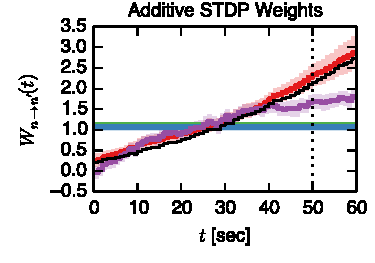
\includegraphics[width=\textwidth]{figures/ch4/fig3_add_nothr_trajectory}    
    \label{fig:fig3_add_nothr_trajectory}
  \end{subfigure}
  \begin{subfigure}[T]{1.45in}
    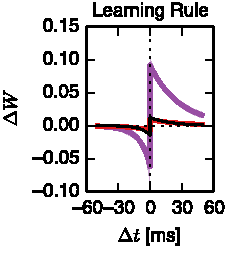
\includegraphics[width=\textwidth]{figures/ch4/fig3_add_nothr_stdp_rule}    
    \label{fig:fig3_add_nothr_stdp_rule}
  \end{subfigure}
  \begin{subfigure}[T]{1.45in}
    \hspace{.1in}
    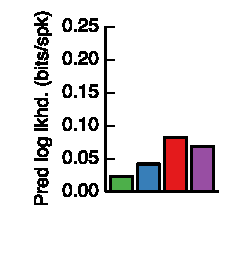
\includegraphics[width=\textwidth]{figures/ch4/fig3_add_nothr_pred_ll2}    
    \label{fig:fig3_add_nothr_pred_ll}
  \end{subfigure}\\
  \vspace{-1.5em}
  \begin{subfigure}[T]{2.4in}
    \flushleft
    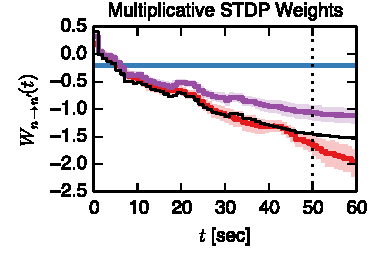
\includegraphics[width=\textwidth]{figures/ch4/fig3_mult_trajectory}    
    \label{fig:fig3_mult_trajectory}
  \end{subfigure}
  \begin{subfigure}[T]{1.45in}
    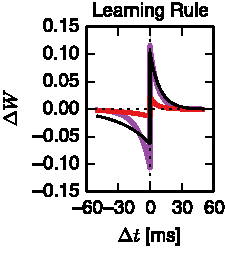
\includegraphics[width=\textwidth]{figures/ch4/fig3_mult_stdp_rule}    
    \label{fig:fig3_mult_stdp_rule}
  \end{subfigure}
  \begin{subfigure}[T]{1.45in}
    \hspace{.1in}
    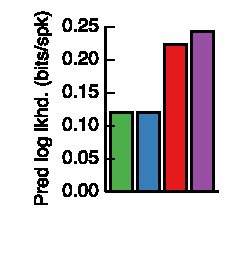
\includegraphics[width=\textwidth]{figures/ch4/fig3_mult_pred_ll}    
    \label{fig:fig3_mult_pred_ll}
  \end{subfigure}\\
  \vspace{-1.9em}
  \begin{subfigure}[T]{\textwidth}
  \centering
  
\includegraphics[height=1.25em]{figures/ch4/fig3_legend}    
  \end{subfigure}
%  \vspace{-1.25em}
  \caption[Synaptic weight trajectories for synthetic data from a
    time-varying GLM]{We fit time-varying weight trajectories to spike
    trains simulated from a GLM with two neurons undergoing no
    plasticity (top row), an additive, unbounded STDP rule (middle),
    and a multiplicative, saturating STDP rule (bottom row). We fit
    the first 50 seconds with four different models: MAP for an
    L1-regularized GLM, and fully-Bayesian inference for a static,
    additive STDP, and multiplicative STDP learning rules.  In all
    cases, the correct models yield the highest predictive log
    likelihood on the final 10 seconds of the dataset.}
  \label{fig:glm_pairs_inference}
\end{figure}

We evaluated our technique with two types of synthetic data. First, we
generated data from our model, with known ground-truth. Second, we
used the well-known simulator NEURON to simulate driven,
interconnected populations of neurons undergoing synaptic
plasticity. For comparison, we show how the sparse, time-varying GLM
compares to a standard GLM with a group LASSO prior on the impulse
response coefficients for which we can perform efficient MAP
estimation.

\subsection{GLM-based simulations}
As a proof of concept, we study a single synapse undergoing a variety
of synaptic plasticity rules and generating spikes according to a
GLM. The neurons also have inhibitory self-connections to mimic
refractory effects. We tested three synaptic plasticity mechanisms: a
static synapse (i.e., no plasticity), the unbounded, additive STDP
rule given by Equation~\ref{eqn:AddSTDP}, and the bounded,
multiplicative STDP rule given by Equation~\ref{eqn:MultSTDP}. For
each learning rule, we simulated 60 seconds of spiking activity at
1kHz temporal resolution, updating the synaptic weights every 1s. The
baseline firing rates were normally distributed with mean~$20$Hz and
standard deviation of~$5$Hz. Correlations in the spike timing led to
changes in the synaptic weight trajectories that we could detect with
our inference algorithm.

% ROC Curve for synapse detection
\begin{figure}[t!]
  \centering
  \vspace{-0.5em}
  \begin{subfigure}[T]{2in}
    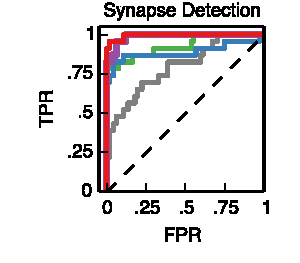
\includegraphics[width=\textwidth]{figures/ch4/fig5_roc_network_1}    
    \label{fig:fig5_roc_network_1}
  \end{subfigure}\hfill
  \begin{subfigure}[T]{3in}
    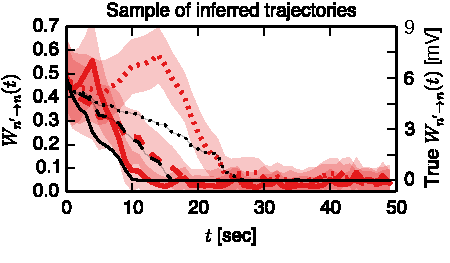
\includegraphics[width=\textwidth]{figures/ch4/fig5_fp_analysis_mv}    
    \label{fig:fig5_fp_analysis}
  \end{subfigure}\\
  \vspace{-1.9em}
  \begin{subfigure}[T]{\textwidth}
  \centering
  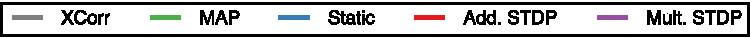
\includegraphics[height=1.25em]{figures/ch4/fig5_legend}    
  \end{subfigure}
%  \vspace{-1em}
%  \vspace{-.5em}
  \caption[Dynamic link prediction on data generated from NEURON]{
    Evaluation of synapse detection on a 60 second spike train
    from a network of 10 neurons undergoing synaptic plasticity with a
    saturating, additive STDP rule, simulated with NEURON. The sparse,
    time-varying GLM with an additive rule outperforms the
    fully-Bayesian model with static weights, MAP estimation with L1
    regularization, and simple thresholding of the cross-correlation
    matrix. }
  \label{fig:pynn_roc}
  \vspace{-1em}
\end{figure}

Figure~\ref{fig:glm_pairs_inference} shows the true and inferred
weight trajectories, the inferred learning rules, and the predictive
log likelihood on ten seconds of held out data for each of the three
ground truth learning rules. When the underlying weights are static
(top row), MAP estimation and static learning rules do an excellent
job of detecting the true weight whereas the two time-varying models
must compensate by either setting the learning rule as close to zero
as possible, as the additive STDP does, or setting the threshold such
that the weight trajectory is nearly constant, as the multiplicative
model does. Note that the scales of the additive and multiplicative
learning rules are not directly comparable since the weight updates in
the multiplicative case are modulated by how close the weight is to
the threshold. When the underlying weights vary (middle and bottom
rows), the static models must compromise with an intermediate
weight. Though the STDP models are both able to capture the
qualitative trends, the correct model yields a better fit and better
predictive power in both cases.

In terms of computational cost, our approach is clearly more expensive
than alternative approaches based on MAP estimation or MLE. We
developed a parallel implementation of our algorithm to capitalize on
conditional independencies across neurons, i.e. for the additive and
multiplicative STDP rules we can sample the weights~${\bW_{*\to n}}$
independently of the weights~${\bW_{*\to n'}}$. On the two neuron
examples we achieve upward of 2 iterations per second (sampling all
variables in the model), and we run our model for 1000
iterations. Convergence of the Markov chain is assessed by analyzing
the log posterior of the samples, and typically stabilizes after a few
hundred iterations. As we scale to networks of ten neurons, our
running time quickly increases to roughly 20 seconds per iteration,
which is mostly dominated by slice sampling the learning rule
parameters. In order to evaluate the conditional probability of a
learning rule parameter, we need to sample the weight trajectories for
each synapse. Though these running times are nontrivial, they are not
prohibitive for networks that are realistically obtainable for optical
study of synaptic plasticity.

\subsection{Biophysical simulations}
Using the biophysical simulator NEURON, we performed two
experiments. First, we considered a network of 10 sparsely
interconnected neurons (28 excitatory synapses) undergoing synaptic
plasticity according to an additive STDP rule. Each neuron was driven
independently by a hidden population of 13 excitatory neurons and 5
inhibitory neurons connected to the visible neuron with probability
0.8 and fixed synaptic weights averaging 3.0 mV. The visible synapses
were initialized close to 6.0 mV and allowed to vary between 0.0 and
10.5 mV. The synaptic delay was fixed at 1.0 ms for all synapses. This
yielded a mean firing rate of 10 Hz among visible neurons. Synaptic
weights were recorded every 1.0 ms.  These parameters were chosen to
demonstrate interesting variations in synaptic strength, and as we
transition to biological applications it will be necessary to evaluate
the sensitivity of the model to these parameters and the appropriate
regimes for the circuits under study.

We began by investigating whether the model is able to accurately
identify synapses from spikes, or whether it is confounded by spurious
correlations.  Figure~\ref{fig:pynn_roc} shows that our approach
identifies the 28 excitatory synapses in our network, as measured by
ROC curve (Add. STDP AUC=${0.99}$), and
%Furthermore, our sparse, time-varying GLM with STDP models outperform
%static models and simple cross-correlation in a synapse detection
%task, as measured by the ROC curve shown on the left.
outperforms static models and cross-correlation.  In the sparse,
time-varying GLM, the probability of an edge is measured by the mean
of~$\bA$ under the posterior, whereas in the standard GLM with MAP
estimation, the likelihood of an edge is measured by area under the
impulse response.

Looking into the synapses that are detected by the time-varying model
and missed by the static model, we find an interesting pattern. The
improved performance comes from synapses that decay in strength over
the recording period. Three examples of these synaptic weight
trajectories are shown in the right panel of
Figure~\ref{fig:pynn_roc}. The time-varying model assigns over 90\%
probability to each of the three synapses, whereas the static model
infers less than a 40\% probability for each synapse.

Finally, we investigated our model's ability to distinguish various
learning rules by looking at a single synapse, analogous to the
experiment performed on data from the
GLM. Figure~\ref{fig:pynn_pairs_inference} shows the results of a
weight trajectory for a synapse under additive STDP with a strict
threshold on the excitatory postsynaptic current. The time-varying GLM
with an additive model captures the same trajectory, as shown in the
left panel. The GLM weights have been linearly rescaled to align with
the true weights, which are measured in millivolts. Furthermore, the
inferred additive STDP learning rule, in particular the time constants
and relative amplitudes, perfectly match the true learning rule.

These results demonstrate that a sparse, time-varying GLM is capable
of discovering synaptic weight trajectories, but in terms of
predictive likelihood, we still have insufficient evidence to
distinguish additive and multiplicative STDP rules.
%We believe this arises from comparing models on the basis of spike
%times alone, using only spontaneous data.
By the end of the training period, the weights have saturated at a
level that almost surely induces postsynaptic spikes. At this point,
we cannot distinguish two learning rules which have both reached
saturation.  This motivates further studies that leverage this
probabilistic model in an optimal experimental design framework,
similar to recent work by \citet{Shababo-2013}, in order to
conclusively test hypotheses about synaptic plasticity.

\begin{figure}[t!]
  \centering
  \vspace{-0.5em}
  % COMMENTING OUT THE STATIC AND MULTIPLICATIVE RESULTS
  \begin{comment}
  \begin{subfigure}[T]{2.4in}
    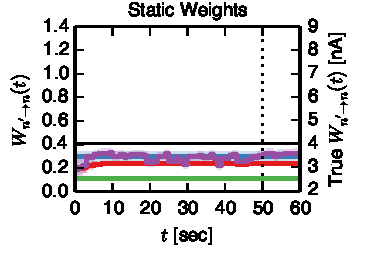
\includegraphics[width=\textwidth]{figures/ch4/fig4_static_trajectory}    
    \label{fig:fig4_static_trajectory}
  \end{subfigure}
  \begin{subfigure}[T]{1.45in}
    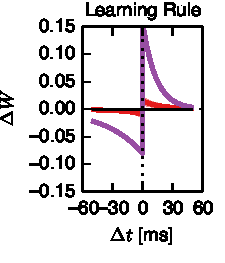
\includegraphics[width=\textwidth]{figures/ch4/fig4_static_stdp_rule}    
    \label{fig:fig4_static_stdp_rule}
  \end{subfigure}
  \begin{subfigure}[T]{1.45in}
    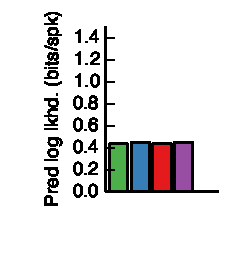
\includegraphics[width=\textwidth]{figures/ch4/fig4_static_pred_ll}    
    \label{fig:fig4_static_pred_ll}
  \end{subfigure} \\
  \vspace{-1.5em}
  \end{comment}
  % ONLY SHOW THE ADDITIVE RESULTS FOR NOW
  \begin{subfigure}[T]{2.4in}
    \flushleft
    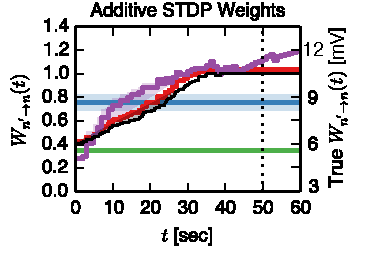
\includegraphics[width=\textwidth]{figures/ch4/fig4_add_thr_trajectory_mv}    
    \label{fig:fig4_add_nothr_trajectory}
  \end{subfigure}
  \begin{subfigure}[T]{1.45in}
    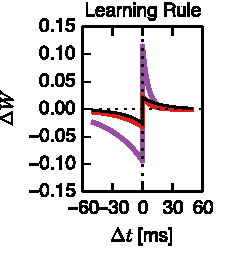
\includegraphics[width=\textwidth]{figures/ch4/fig4_add_thr_stdp_rule}    
    \label{fig:fig4_add_nothr_stdp_rule}
  \end{subfigure}
  \begin{subfigure}[T]{1.45in}
    \hspace{.1in}
    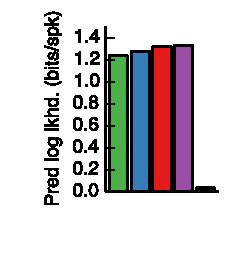
\includegraphics[width=\textwidth]{figures/ch4/fig4_add_thr_pred_ll}    
    \label{fig:fig4_add_nothr_pred_ll}
  \end{subfigure}\\
  \vspace{-1.5em}
  % COMMENTING OUT THE STATIC AND MULTIPLICATIVE RESULTS
  \begin{comment}
  \begin{subfigure}[T]{2.4in}
    \flushleft
    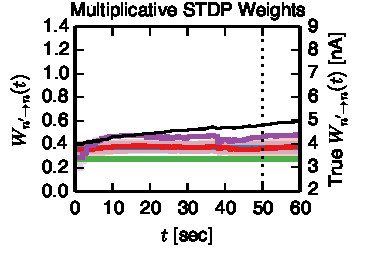
\includegraphics[width=\textwidth]{figures/ch4/fig4_mult_stdp_trajectory}    
    \label{fig:fig4_mult_stdp_trajectory}
  \end{subfigure}
  \begin{subfigure}[T]{1.45in}
    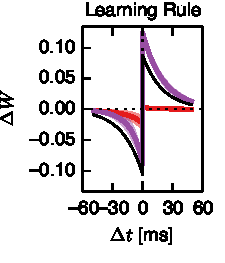
\includegraphics[width=\textwidth]{figures/ch4/fig4_mult_stdp_rule}    
    \label{fig:fig4_mult_stdp_rule}
  \end{subfigure}
  \begin{subfigure}[T]{1.45in}
    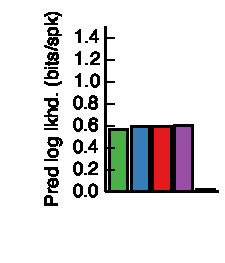
\includegraphics[width=\textwidth]{figures/ch4/fig4_mult_stdp_pred_ll}    
    \label{fig:fig4_mult_stdp_pred_ll}
  \end{subfigure}\\
%  \vspace{-1.75em}
  \vspace{-.75em}
  \end{comment}
  % LEGEND
  \begin{subfigure}[T]{\textwidth}
  \centering
  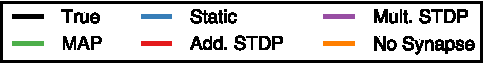
\includegraphics[height=2em]{figures/ch4/fig4_legend}    
  \end{subfigure}
  %
%  \vspace{-1em}
  \caption[Synaptic weight trajectories for data generated from NEURON]{
    Analogously to Figure~\ref{fig:glm_pairs_inference}, a sparse,
    time-varying GLM can capture the weight trajectories and learning
    rules from spike trains simulated by NEURON. Here an excitatory
    synapse undergoes additive STDP with a hard upper bound on the
    excitatory postsynaptic current. The weight trajectory inferred by
    our model with the same parametric form of the learning rule
    matches almost exactly, whereas the static models must compromise
    in order to capture early and late stages of the data, and the
    multiplicative weight exhibits qualitatively different
    trajectories. Nevertheless, in terms of predictive log likelihood,
    we do not have enough information to correctly determine the
    underlying learning rule. Potential solutions are discussed in the
    main text.}
  \label{fig:pynn_pairs_inference}
\end{figure}


\section{Discussion}
Motivated by the advent of optical tools for interrogating networks of
synaptically connected neurons, which make it possible to study
synaptic plasticity in novel ways, we have extended the GLM to model a
sparse, time-varying synaptic network, and introduced a fully-Bayesian
inference algorithm built upon particle MCMC. Our initial results
suggest that it is possible to infer weight trajectories for a variety
of biologically plausible learning rules.

 A number of interesting questions remain as we look to apply these
 methods to biological recordings. We have assumed access to precise
 spike times, though extracting spike times from optical recordings
 poses inferential challenges of its own. Solutions like those of
 \citet{Vogelstein-2009} could be incorporated into our probabilistic
 model.  Computationally, particle MCMC could be replaced with
 stochastic EM to achieve improved performance \cite{Lindsten-2012},
 and optimal experimental design could aid in the exploration of
 stimuli to distinguish between learning rules.
%With this foundation, we intend to apply our methods to biological
%recordings and use optimal experimental design \cite{Shababo-2013} to
%design stimuli that will yield maximal information about the
%underlying learning rules.
Beyond these direct extensions, this work opens up potential to infer
latent state spaces with potentially nonlinear dynamics and
non-Gaussian noise, and to infer learning rules at the synaptic or
even the network level.

